%
% Presentation for my talk at GopherCon Russia 2018
% Requires ITooLabs Beamer style to compile (git.itoolabs.com:growler/itoolabs-beamer)
% (which is too messy to open source it anyway)
%
% (c) Alexey Naidyonov 2018
% License CC-BY 3.0
%
\documentclass[
   12pt, background = clouds, fonts = fira, 4k
]{itoolabs-beamer}

% minted setup
\usepackage[outputdir=\outputdir]{minted}
\usepackage{mdframed}

\newcommand{\inputcode}[3][]{%
  \begin{mdframed}[innerleftmargin=3pt, linewidth=0.2pt, linecolor=black!95, hidealllines=true, leftline=true]%
    \inputminted[breaklines, tabsize=4, numbersep=6pt, linenos, fontsize=\scriptsize,#1]{#2}{code/#3}%
  \end{mdframed}%
}

\newenvironment{code}[1]
{\VerbatimEnvironment%
 \begin{mdframed}[innerleftmargin=3pt, linewidth=0.2pt, linecolor=black!95, hidealllines=true, leftline=true]%
    \begin{minted}[breaklines, autogobble, tabsize=4, numbersep=6pt, linenos, fontsize=\scriptsize]{#1}}%
   {\end{minted}%
 \end{mdframed}%
}%

\renewcommand{\theFancyVerbLine}{\ttfamily \textcolor{black!40}{\tiny \arabic{FancyVerbLine}}}
%

% a poor man's sequence diagram
% a poor man's sequence diagram
\usetikzlibrary{arrows,arrows.meta,calc,positioning,backgrounds}
\tikzset{>={Stealth[length=1.2ex, width=.6ex]}}

\makeatletter
\newenvironment{seqdiag}[2][]{%
\definecolor{diagramcolor}{rgb}{0.62,0.00,0.184}%
\pgfkeys{/sd/.cd,%
  height/.initial=9,%
  #1}%
% \msg{Position}{From}{To}{Comment}
\newcommand{\msg}[4]{%
  \def\@srcw{\csname line@width@##2\endcsname}%
  \def\@dstw{\csname line@width@##3\endcsname}%
  \draw let \p1=(line@origin@##2),%
            \p2=(line@origin@##3),%
            \p3=($(curpos)+(0,##1)$),
            \n1={(\x1 < \x2) ? (\x1 + \@srcw) : (\x1 - \@srcw)},%
            \n2={(\x1 < \x2) ? (\x2 - \@dstw) : (\x2 + \@dstw)}%
        in%
            [->,draw=diagramcolor, line cap=rect, line width=0.5pt]%
            (\n1,\y3) -- node[midway, fill=white] {##4} (\n2,\y3)%
            coordinate (curpos) at (\p3);%
}%
\newcommand{\proc}[4]{%
  \draw let
        \p1=($(line@origin@##2)-(2ex,0)$),
        \p2=($(line@origin@##3)+(2ex,0)$),
        \p3=($(curpos) + (0,##1)$)
   in
        [draw, line width=0.5pt, double distance=0.5ex]
        (\x1,\y3) -- node[midway, fill=white] {##4} (\x2,\y3)
        coordinate (curpos) at (\p3);%
}%
\newcommand{\enclose}[3]{
  \begin{scope}[on background layer]
    \path let \p1=(current bounding box.north), \p2=(current bounding box.south) in
          [draw, dotted, thin] (##1,\y1) rectangle (##2,\y2)
          (##1, \y1) -- node[below] {##3} (##2,\y1);
  \end{scope}
}
% \instance{position}{Name}{Comment}
\newcommand{\instance}[3]{%
  \begin{scope}[yscale = 1, local bounding box=inst@##2]%
    \node[draw] at (##1cm, 0) {##2};%
  \end{scope}%
  \path let \p1=(inst@##2.south) in coordinate (line@origin@##2) at (\x1, 2ex);%
}
% \actor{position}{name}{comment}
\newcommand{\actor}[3]{%
  \begin{scope}[yscale = 1, inner sep=0, local bounding box=inst@##2]%
    \node (name) at (##1cm, 0) {##2};%
    \node[above=3pt of name] {##3};%
  \end{scope}%
  \path let \p1=(inst@##2.south) in coordinate (line@origin@##2) at (\x1, 2ex);%
}%
\newcommand{\eventline}[1]{
  \expandafter\def\csname line@width@##1\endcsname{0.25pt}%
  \pgfkeysgetvalue{/sd/height}{\@sd@height}%
  \path let \p1=(line@origin@##1)
        in
            coordinate (origin) at (\p1)
            coordinate (finish) at ($(\p1) + (0,\@sd@height)$);%
  \draw[draw=diagramcolor, line width=0.5pt, line cap=rect, dashed] (origin) -- (finish);%
}%
\newcommand{\eventthread}[3]{
  \expandafter\def\csname line@width@##1\endcsname{2.25pt}%
  \pgfkeysgetvalue{/sd/height}{\@sd@height}%
  \path let \p1=(line@origin@##1)
        in
            coordinate (origin) at (\p1)
            coordinate (start) at ($(\p1) + (0,##2cm)$)
            coordinate (stop) at ($(\p1) + (0,##3cm)$)
            coordinate (finish) at ($(\p1) + (0,\@sd@height)$)
            coordinate (left) at ($(start) - (2pt,0)$)
            coordinate (right) at ($(stop) + (2pt,0)$);
  \draw[diagramcolor, line width=0.5pt, line cap=rect, dashed] (origin) -- (start);%
  \draw[diagramcolor, line width=0.5pt] (left) rectangle (right);
  \draw[diagramcolor, line width=0.5pt, line cap=rect, dashed] (stop) -- (finish);%
}%
\begin{tikzpicture}[yscale=-1]%
  \path coordinate (curpos) at (0,2ex);
  #2%
}{%
\end{tikzpicture}%
}
\makeatother
%%% Local Variables:
%%% mode: latex
%%% TeX-master: t
%%% End:


\setbeameroption{hide notes}
\setbeamertemplate{itemize item}{\color{ITooLabsOrange}\textbullet}

\mode<presentation>{}

\simplefootline%

\title{Embedding JavaScript into Go}
\author{Alexey Naidyonov}
\event{GopherCon Russia 2018}
\date[17.03.2018]{Mar 17 2018}

\eventlogo{\includegraphics{gophers/gophercon-russia.pdf}}
\setbeamertemplate{title event logo}{
  
\includegraphics[keepaspectratio,width=.1\paperwidth]{gophers/gopher-itoolabs.pdf}%
  \hfill%
  \includegraphics[keepaspectratio,width=.11\paperwidth]{gophers/gophercon-russia.pdf}%
  \par%
}

\begin{document}

\begin{frame}[plain]\titlepage\end{frame}

\begin{frame}[c]
  \frametitle{ITooLabs PaaS}
  \begin{columns}[widths={3,2}]
    \begin{column}
      \begin{itemize}
      \item White-label cloud PBX
      \item ITooLabs cloud or telco's on-premises
      \item Branded UIs \& B/OSS integration
      \item 80+ telcos onboard
      \item 15 000+ SMBs total
      \item 1 500+ (and growing) new subscribers monthly
      \item 300+ mln.\ minutes of calls total in 2017
      \end{itemize}
    \end{column}
    \begin{column}
      \centering\includegraphics[keepaspectratio, width=\textwidth]{itoolabs-service.png}%
    \end{column}
  \end{columns}
\end{frame}

\begin{frame}[c]
  \centering\Huge{What's the fuss?}
\end{frame}

\def\ActorAlice{\actor{0}{Alice}{
\includegraphics[height=5ex]{gophers/gopher-alice.pdf}}}
\def\ActorBob{\actor{12}{Bob}{\scalebox{-1}[1]{
\includegraphics[height=5ex]{gophers/gopher-bob.pdf}}}}

\begin{frame}
  \frametitle{Call model}
  \centering\scriptsize
  \begin{seqdiag}[height=5.5cm]
    \ActorAlice%
    \ActorBob%
    \eventline{Alice}
    \eventline{Bob}
    \msg{0.2}{Alice}{Bob}{Call}
    \msg{0.8}{Bob}{Alice}{Ringing}
    \msg{0.8}{Bob}{Alice}{Answered}
    \msg{0.8}{Alice}{Bob}{OK}
    \proc{0.9}{Alice}{Bob}{talking}
    \msg{0.9}{Bob}{Alice}{Bye}
    \msg{0.8}{Alice}{Bob}{OK}
  \end{seqdiag}
\end{frame}

\begin{frame}
  \frametitle{Call model}
  \centering\scriptsize
  \begin{seqdiag}[height=5.5cm]
    \ActorAlice%
    \instance{6}{PBX}{PBX}
    \ActorBob%
    \eventline{Alice}
    \eventline{PBX}
    \eventline{Bob}
    \msg{0.2}{Alice}{PBX}{Call}
    \msg{0.1}{PBX}{Bob}{Call}
    \msg{0.8}{Bob}{PBX}{Ringing}
    \msg{0.1}{PBX}{Alice}{Ringing}
    \msg{0.8}{Bob}{PBX}{Answered}
    \msg{0.1}{PBX}{Alice}{Answered}
    \msg{0.8}{Alice}{PBX}{OK}
    \msg{0.1}{PBX}{Bob}{OK}
    \proc{0.6}{Alice}{Bob}{talking}
    \msg{0.6}{Bob}{PBX}{Bye}
    \msg{0.1}{PBX}{Alice}{Bye}
    \msg{0.8}{Alice}{PBX}{OK}
    \msg{0.1}{PBX}{Bob}{OK}
  \end{seqdiag}
\end{frame}

\begin{frame}
  \frametitle{Call model}
  \centering\scriptsize
  \begin{seqdiag}[height=5.5cm]
    \ActorAlice%
    \actor{4.5}{T1}{
\includegraphics[height=5ex]{gophers/gopher-itoolabs.pdf}}
    \actor{7.5}{T2}{\scalebox{-1}[1]{
\includegraphics[height=5ex]{gophers/gopher-itoolabs.pdf}}}
    \ActorBob%
    \eventline{Alice}
    \eventthread{T1}{0.2}{5.1}
    \eventthread{T2}{0.3}{5.2}
    \eventline{Bob}
    \enclose{3.9}{8.1}{PBX}
    \msg{0.2}{Alice}{T1}{Call}
    \msg{0.1}{T1}{T2}{spawn}
    \msg{0.1}{T2}{Bob}{Call}
    \msg{0.6}{Bob}{T2}{Ringing}
    \msg{0.1}{T2}{T1}{provisional}
    \msg{0.1}{T1}{Alice}{Ringing}
    \msg{0.6}{Bob}{T2}{Answered}
    \msg{0.1}{T2}{T1}{connected}
    \msg{0.1}{T1}{Alice}{Answered}
    \msg{0.6}{Alice}{T1}{OK}
    \msg{0.1}{T1}{T2}{confirmed}
    \msg{0.1}{T2}{Bob}{OK}
    \proc{0.7}{Alice}{Bob}{talking}
    \msg{0.7}{Bob}{T2}{Bye}
    \msg{0.1}{T2}{T1}{disconnect}
    \msg{0.1}{T1}{Alice}{Bye}
    \msg{0.6}{Alice}{T1}{OK}
    \msg{0.1}{T1}{T2}{disconnected}
    \msg{0.1}{T2}{Bob}{OK}
  \end{seqdiag}
\end{frame}

\begin{frame}[c]
  \frametitle{ITooLabs Centrex}
  \centering
  \begin{minipage}{.33\textwidth}
    \Large
    \begin{itemize}
    \item Easy to develop
    \item Easy to deploy
    \item Easy to scale
    \end{itemize}
  \end{minipage}
\end{frame}

\begin{frame}[c]
  \frametitle{ITooLabs Centrex}
  \begin{figure}
    \resizebox{!}{.9\textheight}{\begin{tikzpicture}[
  cisco icon/.style args={#1,#2}{
    node contents={\includegraphics[keepaspectratio, width=6ex]{cisco/#1.pdf}},%
    label={[label position=below, shift={(0,1ex)}, align=center]#2}%
  }]%
  \definecolor{oam}{rgb}{0.000,0.180,1.000}
  \definecolor{pnet}{rgb}{0.663,0.482,0.298}
  \node (router) [cisco icon={router,}];
  \node (lb1) [above right=3cm and 3cm of router, cisco icon={lb,LB}];
  \node (lb2) [below=1.5cm of lb1, cisco icon={lb,LB}];
  \node (fe1) [right=2cm of lb1, cisco icon={fe,Front End 1}];
  \node (fe2) [right=2cm of lb2, cisco icon={fe,Front End N}];
  \node (mg1) [below=1.5cm of fe2, cisco icon={mg,Media\\Processor 1}];
  \node (mg2) [below=1.5cm of mg1, cisco icon={mg,Media\\Processor N}];
  \node (be1) [right=2cm of fe2, cisco icon={be,Back End 1}];
  \node (be2) [right=2cm of mg1, cisco icon={be,Back End N}];
  \node at ($(fe1.south)!0.7!(fe2.north)$) {\Large\ldots};
  \node at ($(be1.south)!0.6!(be2.north)$) {\Large\ldots};
  \node at ($(mg1.south)!0.8!(mg2.north)$) {\Large\ldots};
  \path let \p1=($(lb1.west)!0.33!(router.east)$),
            \p2=($(lb1.east)!0.5!(fe1.west)$),
            \p3=($(fe1.east)!0.5!(be1.west)$) in
        coordinate (oamn) at ($(\p3|-fe1.north) + (0,.2cm)$)
        coordinate (oams) at ($(\p3|-mg2.south) - (0,.8cm)$)
        coordinate (pnet1n) at (\p2|-oamn)
        coordinate (pnet1s) at ($(\p2|-fe2.south) - (0,.5cm)$)
        coordinate (pnet2n) at (\p1|-oamn)
        coordinate (pnet2s) at (\p1|-pnet1s)
        coordinate (pnet3n) at ($(\p2|-mg1.north) + (0,.2cm)$)
        coordinate (pnet3s) at (\p2|-oams);
  \draw[very thick, oam]
        (oamn) -- (oams)
        (fe1.east) -- (oamn|-fe1.east)
        (fe2.east) -- (oamn|-fe2.east)
        (be1.west) -- (oamn|-be1.west)
        (be2.west) -- (oamn|-be2.west)
        (mg1.east) -- (oamn|-mg1.east)
        (mg2.east) -- (oamn|-mg2.east);
  \draw[very thick, pnet]
        let \p1=($(pnet2n)!0.5!(pnet2s)$),
            \p2=($(pnet3n)!0.5!(pnet3s)$) in
        (pnet1n) -- (pnet1s)
        (pnet2n) -- (pnet2s)
        (pnet3n) -- (pnet3s)
        (router.north) -- (router.north|-\p1) -- node[black,above]{Signalling} node[black,below]{(SIP)} (\p1)
        (router.south) -- (router.south|-\p2) -- node[black,above]{Media} node[black,below]{(RTP)} (\p2)
        (lb1.west) -- (pnet2n|-lb1.west)
        (lb2.west) -- (pnet2n|-lb2.west)
        (lb1.east) -- (pnet3n|-lb1.east)
        (lb2.east) -- (pnet3n|-lb2.east)
        (fe1.west) -- (pnet1n|-fe1.west)
        (fe2.west) -- (pnet1n|-fe2.west)
        (mg1.west) -- (pnet1n|-mg1.west)
        (mg2.west) -- (pnet1n|-mg2.west);
  \draw [<->,>=Stealth, very thick] (router.west) -- ++(-2cm,0);
\end{tikzpicture}
%%% Local Variables:
%%% mode: latex
%%% End:
}
  \end{figure}
\end{frame}

\begin{frame}[c,fragile]
  \frametitle{ITooLabs Centrex}
  \inputcode{go}{greeter.go}
\end{frame}

\begin{frame}[c]
  \frametitle{ITooLabs Centrex}
  \begin{description}[\mintinline{javascript}{SendEvent(tid, what, param)}]
  \item[\mintinline{javascript}{Spawn('task', param)}] spawns new task and returns \emph{tid}
  \item[\mintinline{javascript}{ParentTask()}] returns \emph{tid} of the parent task
  \item[\mintinline{javascript}{ThisTask()}] returns \emph{tid} of the current task
  \item[\mintinline{javascript}{SendEvent(tid, what, param)}] sends \emph{what} with \emph{param} to \emph{tid}
  \item[\mintinline{javascript}{ReadInput()}] reads first event from the task's queue
  \end{description}
\end{frame}

\begin{frame}[c]
  \centering\huge{First try: embedding Lua 5.1 C VM}
\end{frame}

\begin{frame}[c,fragile]
  \frametitle{Lua Call Processing Task}
  \inputcode{lua}{greeter.lua}
\end{frame}

\begin{frame}[c]
  \frametitle{Issues}
  \large\begin{itemize}
  \item CGo calls were way too slow (and still are)
    \pause%
  \item Too much hassle with conversions
    \pause%
  \item Incomprehensible stack traces for non-terminal calls
  \end{itemize}
\end{frame}

\begin{frame}[c]
  \centering
  {\huge Second try: embedding Otto}\\
  \vskip1cm%
  {\Large JavaScript interpreter in Go (\href{https://github.com/robertkrimen/otto}{github.com/robertkrimen/otto})}
\end{frame}

\begin{frame}[c,fragile]
  \frametitle{ECMAScript Call Processing Task}
  \inputcode{javascript}{greeter.js}
\end{frame}

\begin{frame}
  \frametitle{Issues}
  \large\begin{itemize}
  \item Gosh, it's soooo SLOW (100x times)
    \pause%
  \item A huge burden on GC
    \pause%
  \end{itemize}
  \begin{center}
    \ldots yet it works! \\
    \vskip1ex%
    \pause%
    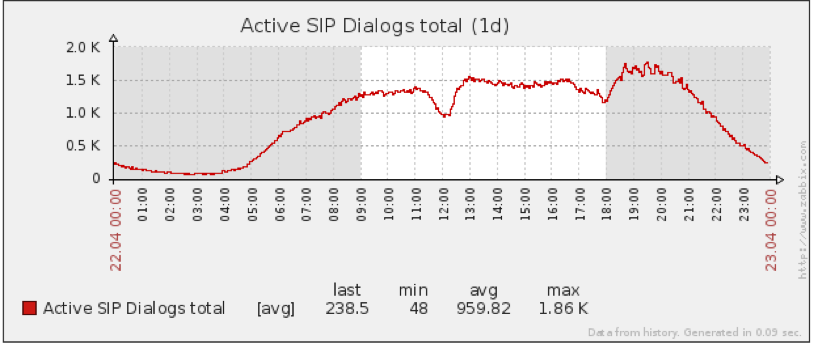
\includegraphics[keepaspectratio, height=.5\textheight]{sip-dialogs-graph.png}
  \end{center}
\end{frame}

\begin{frame}[c]
  \centering
  {\huge Third try: rewriting Otto}\\
  \vskip2ex%
  {\Large Meet Goja! (\href{https://github.com/dop251/goja}{github.com/dop251/goja})}
  \vskip2ex%
  \large\begin{itemize}
  \item byte code VM
    \pause%
  \item lots of improvements
    \pause%
  \item 10x-30x times faster than Otto\\
    (still slow for computation intensive tasks, but pretty much fine for us)
  \end{itemize}
\end{frame}

\begin{frame}[fragile]
  \frametitle{ECMAScript Call Processing Tasks}
  \begin{columns}[T,two]
    \begin{column}
      \inputcode{javascript}{ingress.js}
    \end{column}
    \begin{column}
      \inputcode{javascript}{egress.js}
    \end{column}
  \end{columns}
\end{frame}

\begin{frame}[c]
  \frametitle{There are still issues\ldots}
  \large\begin{itemize}
  \item Might be surprisingly slow\\
    (don't try to iterate over 100k+ user accounts)
    \pause%
  \item Sharing data is an easy way to shoot oneself in the foot\\
    (we had to got rid of it)
    \pause%
  \item Still huge burden on GC\\
    (looking forward to generational GC!)
  \end{itemize}
\end{frame}

\begin{frame}[c]
  \frametitle{\ldots but advantages are huge}
  \large\begin{itemize}
  \item Weekly (daily, hourly) deploys\\
    \pause%
    {\normalsize\mintinline{shell}{installapp default git "git@git.site:app/app" 0a3124f}}%
    \pause%
  \item Multiple applications on the same running service%
    \pause%
  \item (last but not least) Same language for UI and Call Control
  \end{itemize}
\end{frame}

\begin{frame}[c]
  \frametitle{Conclusions}
  \large\begin{itemize}
  \item Embedding would suit you as long as \ldots
    \pause%
    \begin{itemize}
    \item some tasks change way too often
      \pause%
    \item these tasks are not computation intensive \ldots
      \pause%
    \item \ldots and most of time just wait for the event
      \pause%
    \end{itemize}
  \item but beware of Garbage Collector!
  \end{itemize}
\end{frame}

\begin{frame}[c]
  \frametitle{Go Scripting Landscape}
  \small\begin{itemize}
  \item \url{https://github.com/robertkrimen/otto} --- (A very basic) ECMAScript interpreter
    \pause%
  \item \url{https://github.com/dop251/goja} --- ECMAScript 5.1 interpreter
    \pause%
  \item \url{https://github.com/Shopify/go-lua} --- Shopify's Go Lua
    \pause%
  \item \url{https://github.com/yuin/gopher-lua} --- Go Lua
    \pause%
  \item \url{https://github.com/mattn/anko} --- Scriptable interpreter for Go
    \pause%
  \item \url{https://neugram.io/} --- A Go scripting with Go Syntax
    \pause%
  \item \ldots Tcl, Scheme, Lisp, Forth, Ruby, \ldots
  \end{itemize}
\end{frame}

\begin{frame}[c]
  \frametitle{Questions?}
  \begin{center}
    \XKCD[height=.75\textheight]{1403-thesis-defense}%
  \end{center}
\end{frame}

\begin{frame}[c]
  \frametitle{Author}
  \begin{columns}[c,widths={2,3}]
    \begin{column}
      Alexey Naidyonov \\
      ITooLabs CEO \\
      \url{https://itoolabs.com} \\
      \href{mailto:anaidyonov@itoolabs.com}{anaidyonov@itoolabs.com} \\
      \href{https://github.com/growler}{github.com/growler}\\
      \href{https://telegram.me/anaidyonov}{@anaidyonov}\\
      \href{tel:+79260024001}{+7 926 002 40 01}
    \end{column}
    \begin{column}
      \centering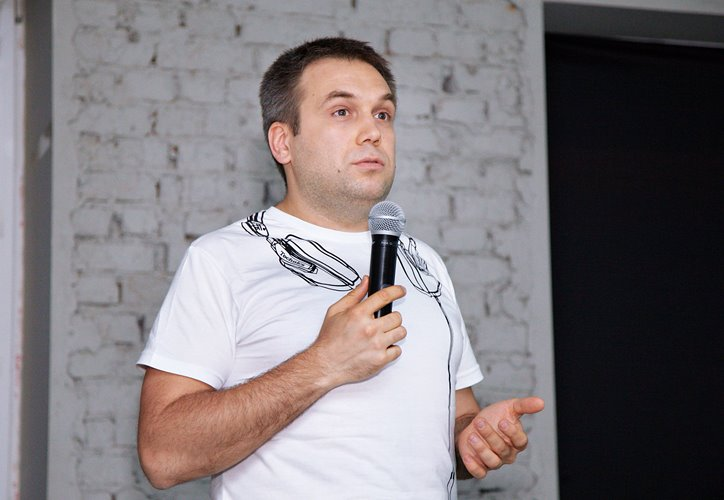
\includegraphics[keepaspectratio, width=.9\textwidth]{author-photo.jpg}
    \end{column}
  \end{columns}
\end{frame}

\end{document}
%%% Local Variables:
%%% mode: latex
%%% TeX-master: t
%%% End:
